\documentclass{beamer}
\usetheme{Madrid}

\usepackage{float}
\usepackage[utf8]{inputenc} % Input encoding
\usepackage[LGR,T1]{fontenc} % Output encoding for Greek and English
%\usepackage[polutonikogreek,english]{babel} % Support for Greek and English
\usepackage{amsmath} % For math support
\usepackage{alphabeta}
\usepackage{graphicx} % Required for inserting images
\usepackage{caption}
\usepackage{subcaption}
\usepackage{amsfonts} % Math fonts
%\usepackage{tocloft} % For table of contents customization
\usepackage[greek,english]{babel}
\usepackage{lmodern}
\usepackage{listings}
\usepackage{xcolor}

% Define Python style for listings
\lstdefinestyle{python}{
    language=Python,
    basicstyle=\ttfamily\footnotesize,
    keywordstyle=\color{blue},
    stringstyle=\color{red},
    commentstyle=\color{cyan},
    showstringspaces=false,
    breaklines=true,
    frame=single,
    tabsize=4,
}


% Title and author details
\title[PR - ML Project]{Project για το μάθημα της Αναγνώρισης Προτύπων και Μηχανικής Μάθησης}
\author[Κιζιρίδης Δ. Μπίλλας Θ.Α.]{Κιζιρίδης Δημήτριος ΑΕΜ: 10539 \\ Μπίλλας Θωμάς Αχιλλέας ΑΕΜ: 10366\\ Ομάδα 33}
\date{Τετάρτη 08 Ιανουαρίου 2025}
\institute[]{Τμήμα Ηλεκτρολόγων Μηχανικών και Μηχανικών Υπολογιστών ΑΠΘ}

\begin{document}
\frame{\titlepage}


\begin{frame}
    \frametitle{Πίνακας Περιεχομένων}
    \small
    \tableofcontents
\end{frame}


\section{Μέρος Α - Εκτίμηση Παραμέτρων με Μέθοδο Μέγιστης Πιθανοφάνειας}
\begin{frame}{Μέρος Α - Εισαγωγή}
    Στόχος του μέρους Α είναι να διαπιστώσουμε κατά πόσο ο δείκτης – αριθμός x, που σχετίζεται με τα μοτίβα συχνότητας και δύναμης πίεσης των πλήκτρων της κονσόλας μπορεί να χρησιμοποιηθεί σε ένα σύστημα ταξινόμησης σχετικά με το στρες των παικτών βιντεοπαιχνιδιών.
    Έτσι, με γνωστή κατανομή πυκνότητας πιθανότητας, καλούμαστε να υλοποιήσουμε έναν ταξινομητή με τη \textbf{Μέθοδο της Μέγιστης Πιθανοφάνειας} για να αξιολογήσουμε το δείκτη x, με βάση δεδομένα που έχουμε αναφορικά με το αν νιώθουν στρες ή όχι οι χρήστες.\\
Στο ερώτημα 1 θα εκτιμηθούν άγνωστες παράμετροι και θα απεικονιστούν τα ζητούμενα διαγράμματα.\\
Στο ερώτημα 2 θα χρησιμοποιηθεί δοθείσα συνάρτηση διάκρισης, θα ταξινομηθούν τα δείγματα που έχουμε και θα διατυπωθούν παρατηρήσεις.

\end{frame}
\begin{frame}{Μέρος Α - Δεδομένα}
Η κατανομή πυκνότητας πιθανότητας που ακολουθεί αυτός ο δείκτης $x$ για τις δύο κλάσεις (χωρίς στρες = κλάση $ω_1$, με στρες = κλάση $ω_2$) είναι:
$$p(x|\theta) = \frac{1}{\pi} \frac{1}{1+(x-\theta)^2}$$ όπου η παράμετρος $\theta$ είναι άγνωστη.\\ 
Έχοντας ένα δείγμα 12 ατόμων και γνωρίζοντας αν δήλωσαν ότι αισθάνθηκαν στρες ή όχι (7 δήλωσαν όχι, 5 δήλωσαν ναι), παίρνουμε τους δείκτες:\\
 $D_1=[ 2.8, -0.4, -0.8, 2.3, -0.3, 3.6, 4.1]$, για την κλάση $ω_1$
 $D_2=[-4.5, -3.4, -3.1, -3.0, -2.3]$, για την κλάση $ω_2$.\\
Δινεται για το ερώτημα 2 η συνάρτηση διάκρισης:
$$g(x) = \log P(x | \hat{\theta}_1) - \log P(x | \hat{\theta}_2) + \log P(\omega_1) - \log P(\omega_2)$$
\end{frame}

\begin{frame}{Μέρος Α - Ερώτημα 1 - Θεωρητική ανάλυση}
    Για να εκτιμήσουμε τις $\hat{\theta}_1, \hat{\theta}_2$ για την παράμετρο $\theta$ μας ζητείται να χρησιμοποιήσουμε τη Μέθοδο Μεγίστης Πιθανοφάνειας, άρα με βάση τη θεωρία πρέπει να βρεθούν οι τιμές που θα μεγιστοποιήσουν τις συναρτήσεις πιθανοφάνειας $p(D_1|\theta)$ και $p(D_2|\theta)$ αντίστοιχα.\\
    Γνωρίζουμε γενικά πως:
    \begin{equation} p(D|\theta) = p(x_1, x_2, \dots, x_N | \theta) = \prod_{n=1}^N p(x_n | \theta)     \label{eq:1}
\end{equation}
    όπου $p(x|\theta) = \frac{1}{\pi} \frac{1}{1+(x-\theta)^2}$ και τα $x_1, x_2, \dots, x_N \in D$.\\
    Έτσι βρίσκουμε τις ζητούμενες τιμές $\hat{\theta}_1, \hat{\theta}_2$ που μεγιστοποιούν τις $p(D_1|\theta)$ και $p(D_2|\theta)$ αντίστοιχα.
\end{frame}

\begin{frame}[fragile]{Μέρος Α - Ερώτημα 1 - Υλοποίηση}
    Προχωρόντας στην υλοποίηση λογαριθμίζουμε τη σχέση (\ref{eq:1}), αφενός γιατί αποτελεί καλή πρακτική για απλοποίηση των υπολογισμών και αφετέρου γιατί μας ζητείται να απεικονίσουμε τις $\log p(\mathcal{D}_1 | \theta)$ και $\log p(\mathcal{D}_2 | \theta)$.
    $$\log p(D|\theta) = \log \prod_{n=1}^N p(x_n | \theta)$$
    Για να πετύχουμε πολύ καλή ακρίβεια στις εκτιμήσεις μας, στην υλοποιήση χρησιμοποιούμε 10000 τιμές στο διάστημα [-5,+5], έχοντας βέβαια επιβεβαίωσει ότι στην περιοχή αυτή βρίσκονται τα ζητούμενα μέγιστα.
     \lstset{style=python}
\begin{lstlisting}
    theta_values = np.linspace(-5, 5, 1000)
\end{lstlisting}
\end{frame}

\begin{frame}{Μέρος Α - Ερώτημα 1 - Υλοποίηση}

% Top row
\begin{minipage}{0.47\textwidth}
    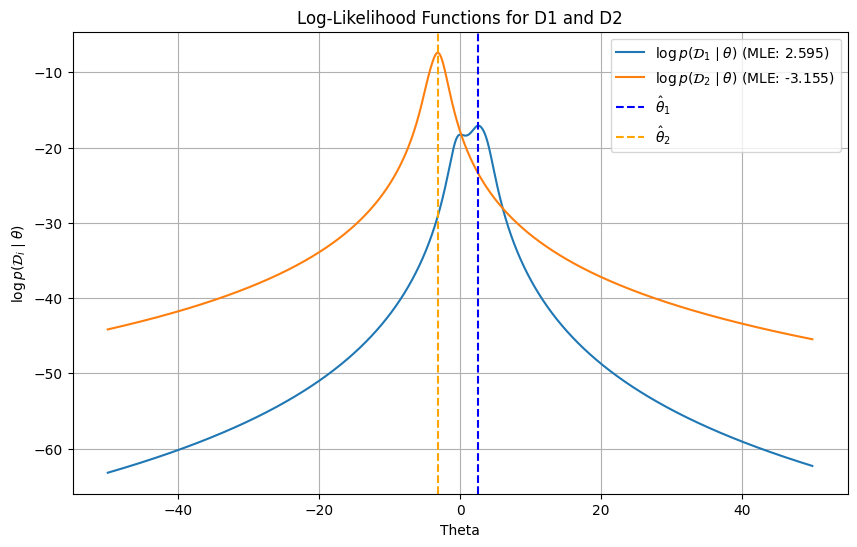
\includegraphics[width=\textwidth]{A/theta estimations-wide.png}
\end{minipage}
\hfill
\begin{minipage}{0.5\textwidth}
Επιβεβαιώνουμε οπτικά την περιοχή στην οποία θα βρεθούν τα μέγιστα, και απεικονίζουμε τις ζητούμενες συναρτήσεις λογαριθμικής πιθανοφάνειας $\log p(\mathcal{D}_1 | \theta)$ και $\log p(\mathcal{D}_2 | \theta)$ συναρτήσει του $\theta$.
\end{minipage}
\vspace{0.5cm} % Add some vertical spacing between the rows
% Bottom row
\begin{minipage}{0.39\textwidth}
Οι ζητούμενες παράμετροι, με ακρίβεια 3 δεκαδικών ψηφίων προκύπτουν:
$$\hat{\theta}_1 = 2.600 \text{ και } \hat{\theta}_1 = -3.159$$
\end{minipage}
\hfill
\begin{minipage}{0.6\textwidth}
    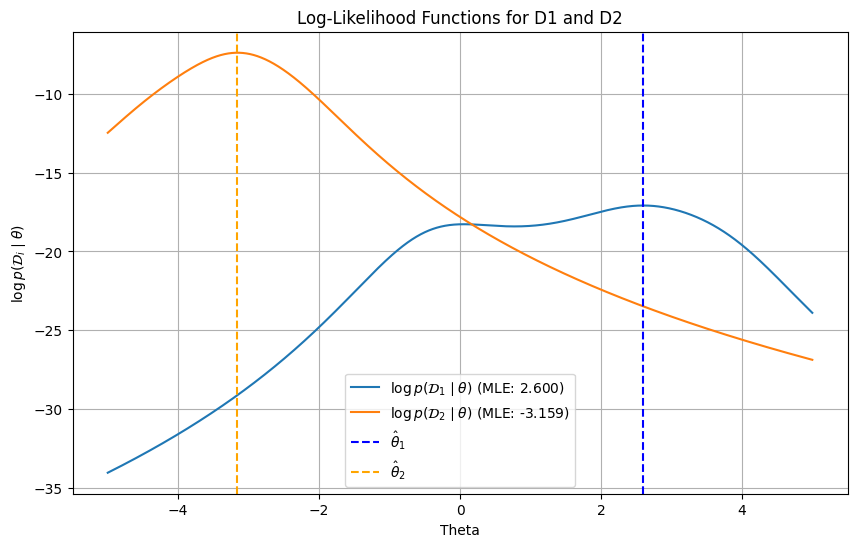
\includegraphics[width=\textwidth]{A/theta estimations.png}
\end{minipage}
\end{frame}

\begin{frame}{Μέρος Α - Ερώτημα 2 - Θεωρητική ανάλυση}
    Στη συνέχεια για την ταξινόμηση θα χρησιμοποιήσουμε τη συνάρτηση διάκρισης που μας δίνεται.
     $$g(x) = \log P(x | \hat{\theta}_1) - \log P(x | \hat{\theta}_2) + \log P(\omega_1) - \log P(\omega_2)$$
Η συνάρτηση και όροι της μας είναι γνώριμοι από τη θεωρία και το γενικό κανόνα του Bayes και γνωρίζουμε - παρατηρούμε πως το πρόσημο της $g(x)$ καθορίζει σε ποια κλάση θα τοποθετηθούν τα δείγματα, δηλαδή για $g(x) > 0 $ το δείγμα τοποθετείται στην κλάση $\omega_1$, ενώ για $g(x) < 0 $ το δείγμα τοποθετείται στην κλάση $\omega_2$.\\
Οι $P(\omega_1)$ και $P(\omega_2)$ προκύπτουν από τον λόγο των δειγμάτων που ανήκουν σε κάθε κλάση προς τον συνολικό αριθμό δειγμάτων που μας δίνονται. Ενώ, οι $\log P(x | \hat{\theta}_1)$ και $ \log P(x | \hat{\theta}_2)$ προκύπτουν από τη δοθείσα σχέση της εκφώνησης.
\end{frame}

\begin{frame}{Μέρος Α - Ερώτημα 2 - Υλοποίηση και Παρατηρήσεις}

\begin{minipage}{0.7\textwidth}
    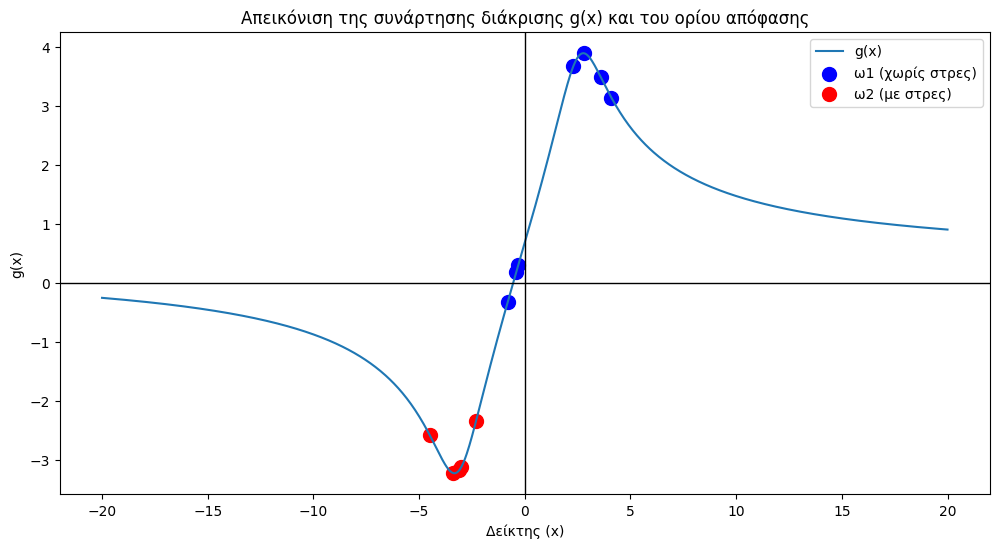
\includegraphics[width=\textwidth]{A/g(x).png}
\end{minipage}
\hfill
\begin{minipage}{0.28\textwidth}
Απεικονίζουμε την $g(x)$ και το όριο απόφασης, καθώς και τα δείγματα που μας δίνονται.
Παρατηρούμε πως ένα δείγμα ($x=-0.8$) ταξινομείται λάθος, ανήκει στην κλάση $\omega_1$ αλλά ταξινομείται στην $\omega_2$.
\end{minipage}
\vspace{0.7cm}
\begin{minipage}{0.6\textwidth}
    Υπενθυμίζουμε πως ο κανόνας απόφασης είναι $\omega_1$ αν $g(x)>0$ και $\omega_2$ αν $g(x)<0$.
\end{minipage}
\end{frame}

%% MEROS B

\section{Μέρος Β - Εκτιμήση Παραμέτρων με Μέθοδο Εκτίμησης κατά Bayes}
\begin{frame}{Μέρος Β - Εισαγωγή}
    Στόχος του μέρους Β είναι να υλοποιήσουμε νέο ταξινομητή για την εκτίμηση της άγνωστης παραμέτρου $\theta$ με τη \textbf{Μέθοδο Εκτίμησης κατά Bayes}. Η prior συνάρτηση πυκνότητας πιθανότητας είναι γνωστή και μας ζητούνται τα εξής:
    \begin{itemize}
        \item Στο ερώτημα 1 να υπολογιστούν και να απεικονιστούν οι εκ των υστέρων πιθανότητες $p(\theta|D_1)$ και $p(\theta|D_2)$.
        \item Στο ερώτημα 2 θα χρησιμοποιηθεί δοθείσα συνάρτηση διάκρισης, θα
ταξινομηθούν τα δείγματα που έχουμε και θα διατυπωθούν
παρατηρήσεις.
    \end{itemize}
\end{frame}
\begin{frame}{Μέρος Β - Δεδομένα}
Από το Μέρος Α, είναι ίδια η $p(x|\theta)$, τα δείγματα $D_1$ και $D_2$, ενώ έχουμε την επιπλέον πληροφορία για την prior συνάρτηση πυκνότητας πιθανότητας, η οποία είναι:
$$p(\theta) = \frac{1}{10\pi} \frac{1}{1 + \left(\frac{\theta}{10}\right)^2}$$
Δινεται για το ερώτημα 2 η συνάρτηση διάκρισης:
$$g(x) = \log P(x | D_1) - \log P(x | D_2) + \log P(\omega_1) - \log P(\omega_2)$$

\end{frame}
\begin{frame}{Μέρος B - Ερώτημα 1 - Θεωρητική ανάλυση}
    Για να εκτιμήσουμε τις $p(\theta|D_1)$ και $p(\theta|D_2)$ έχοντας το γνωστό μοντέλο και με βάση τη θεωρία θα χρησιμοποιήσουμε τη γνωστή από το μάθημα σχέση:
    $$p(\theta \mid D) = \frac{p(D \mid \theta)p(\theta)}{\int p(D \mid \theta)p(\theta) \, d\theta}$$
    όπου $p(D \mid \theta) = \prod_{n=1}^{N} p(x_n \mid \theta)$, και μπορεί να υπολογιστεί όπως στο Μέρος Α. \\
    Οι $p(\theta)$ υπολογίζονται από τη σχέση της εκφώνησης.
\end{frame}
\begin{frame}[fragile]{Μέρος B - Ερώτημα 1 - Υλοποίηση}
    Προχωρώντας στην υλοποίηση, υπολογίζουμε το ζητούμενο με τον κανόνα του Bayes και καθ' υπόδειξιν της εκφώνησης θα χρησιμοποίησουμε κανόνα τραπεζίου για να υπολογίσουμε το ολοκλήρωμα στην έκφραση των $p(\theta|D)$.
        \lstset{style=python}
\begin{lstlisting}
def integralTrapezoid(self, f:np.array, dx:float) -> float:
    return np.sum((f[1:] + f[:-1]) / 2 * dx)
\end{lstlisting} 

\begin{lstlisting}
def calculate_posterior(self, D, thetas):
    dtheta = thetas[1] - thetas[0]
    probs_x_theta = np.array([self.likelihood(D, theta) for theta in thetas])
    probs_D_theta = np.prod(probs_x_theta, axis=1)
    probs_theta = self.prior(thetas)
    integral = self.integralTrapezoid(probs_D_theta * probs_theta, dtheta)
    posterior = (probs_D_theta * probs_theta) / integral
    return posterior
\end{lstlisting}
\end{frame}
\begin{frame}[fragile]{Μέρος B - Ερώτημα 1 - Υλοποίηση}
% Top row
\begin{minipage}{0.47\textwidth}
    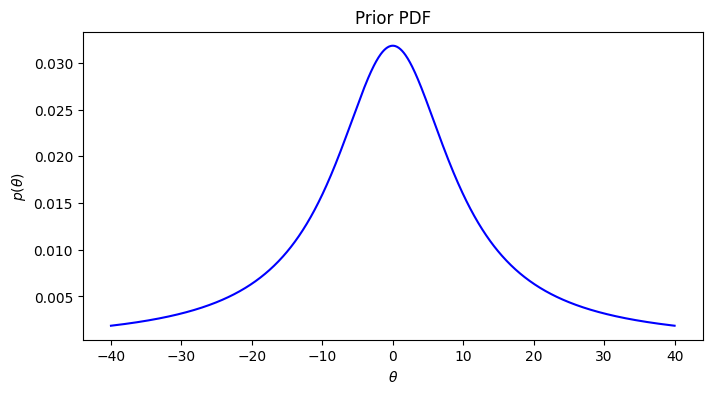
\includegraphics[width=\textwidth]{B/prior pdf.png}
\end{minipage}
\hfill
\begin{minipage}{0.5\textwidth}
Απεικονίζουμε την prior $p(\theta)$, αφού είναι γνωστή συνάρτηση από την εκφώνηση, στο διάστημα [-40,+40] και χρησιμοποιούμε 1000 τιμές για είναι πλήρως εμφανές το σχήμα της.
\end{minipage}
\vspace{0.5cm} % Add some vertical spacing between the rows
% Bottom row
\begin{minipage}{0.39\textwidth}
Απεικονίζουμε τις ζητούμενες εκ των υστέρων πυκνότητες πιθανότητες $p(\theta|D_1)$ και $p(\theta|D_2)$ στο διάστημα [-20,+20] και χρησιμοποιώντας 1000 δείγματα.
\end{minipage}
\hfill
\begin{minipage}{0.6\textwidth}
    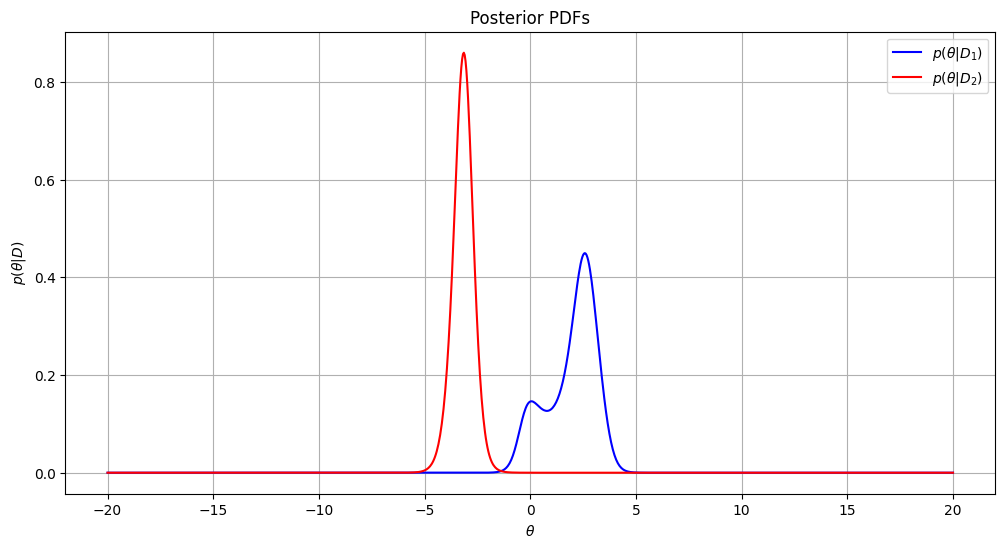
\includegraphics[width=\textwidth]{B/posterior pdfs.png}
\end{minipage}
\end{frame}
\begin{frame}{Μέρος B - Ερώτημα 1 - Υλοποίηση - Παρατηρήσεις}
Με βάση τα ζητούμενα διαγράμματα μπορούμε να εξάγουμε τις εξής παρατηρήσεις:
\begin{itemize}
    \item Οι εκ των υστέρων πυκνότητες πιθανότητας παρουσιάζουν υψηλή συγκέντρωση γύρω από τις πιο πιθανές τιμές των παραμέτρων, με τη μέγιστη τιμή να βρίσκεται κοντά στα σημεία που βρέθηκε και στο μέρος Α, χρησιμοποιώντας τη μέθοδο της Μέγιστης Πιθανοφάνειας. Ειδικότερα για την κλάση $\omega_2$ η εκτίμηση της παραμέτρου είναι με πολύ μεγάλη πιθανότητα.
    \item Από την εκ των προτέρων συνάρτηση πυκνότητας πιθανότητας δε μπορούμε να εξάγουμε κάποια πληροφορία, καθώς τα δεδομένα δεν την επηρεάζουν.
    \item Όπως είδαμε και στη θεωρία έχουμε "μετατρέψει" την εκτίμηση μας σε μια πιο ακριβή αφού έχουμε την πληροφορία των δεδομένων μας (a-posteriori) σε σχέση με πριν τα παρατηρήσουμε (a-priori).
\end{itemize}
\end{frame}
\begin{frame}{Μέρος B - Ερώτημα 2 - Θεωρητική Ανάλυση}
    Στη συνέχεια για την ταξινόμηση θα χρησιμοποιήσουμε τη συνάρτηση διάκρισης που μας δίνεται.
     $$g(x) = \log P(x | D_1) - \log P(x | D_2) + \log P(\omega_1) - \log P(\omega_2)$$
Η συνάρτηση και όροι της μας είναι γνώριμοι από τη θεωρία και το γενικό κανόνα του Bayes και έτσι υπολογίζουμε την $P(x|D)$ από τη γνωστή σχέση:
$$p(x|D) = \int p(x |\theta) p(\theta | D) \, d\theta$$
Οι $P(\omega_1)$ και $P(\omega_2)$ προκύπτουν όπως στο μέρος Α από τον λόγο των δειγμάτων που ανήκουν σε κάθε κλάση προς τον συνολικό αριθμό δειγμάτων που μας δίνονται.\\
Επιπλέον παρατηρούμε - γνωρίζουμε πως το πρόσημο της $h(x)$ καθορίζει σε ποια κλάση θα τοποθετηθούν τα δείγματα, δηλαδή για $h(x) > 0 $ το δείγμα τοποθετείται στην κλάση $\omega_1$, ενώ για $h(x) < 0 $ το δείγμα τοποθετείται στην κλάση $\omega_2$.
\end{frame}
\begin{frame}{Μέρος Β - Ερώτημα 2 - Υλοποίηση και Παρατηρήσεις}
\begin{minipage}{\textwidth}
\begin{figure}
    \centering
    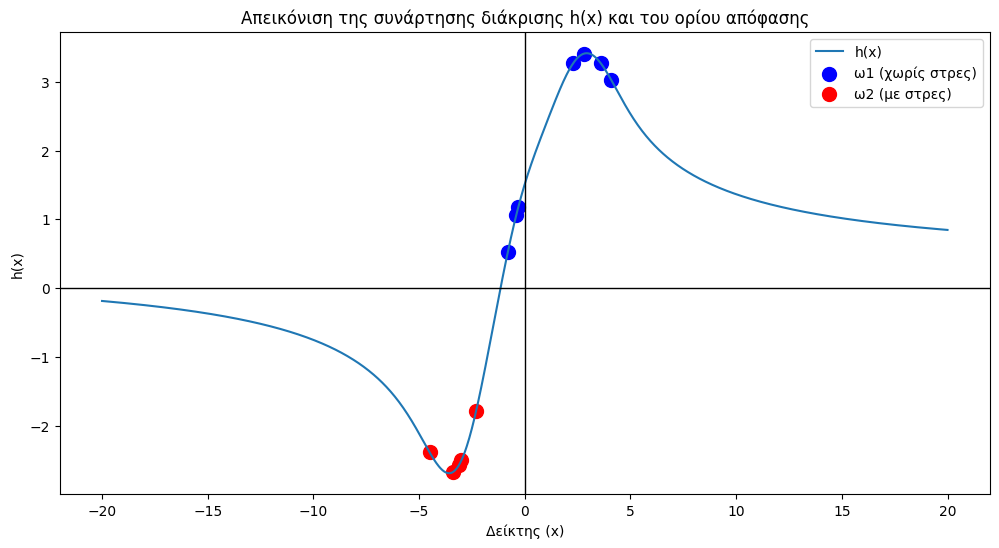
\includegraphics[width=0.88\textwidth]{B/h(x).png}   
\end{figure}
\end{minipage}
\begin{minipage}{\textwidth}
 Απεικονίζουμε την $h(x)$ και το όριο απόφασης, καθώς και τα δείγματα που μας δίνονται.
Παρατηρούμε πως όλα τα δείγματα ταξινομούνται σωστά. Υπενθυμίζουμε πως ο κανόνας απόφασης είναι $\omega_1$ αν $h(x)>0$ και $\omega_2$ αν $h(x)<0$.
\end{minipage}
\end{frame}
\begin{frame}{Μέρος Β - Σύγκριση Μέγιστης Πιθανοφάνειας και Εκτίμησης κατά Bayes}
Έχοντας απεικονίσει τα όρια απόφασης και για τους δύο ταξινομητές, αλλά και τις $g(x)$ και $h(x)$ μπορούμε να εξάγουμε μερικά κρίσιμα συμπεράσματα:
\begin{itemize}
    \item Τα όρια απόφασης έχουν την ίδια μορφολογία και μοιάζουν αρκετά χωρίς όμως να είναι ακριβώς ίδια.
    \item Η εκτίμηση κατά Bayes παρουσιάζει καλύτερα αποτέλεσματα στο συγκεκριμένο πρόβλημα αφού ταξινομεί ορθά όλα τα δείγματα, σε αντίθεση με τον ταξινομητή Μέγιστης Πιθανοφάνειας που ταξινομεί ένα λάθος.
    \item Όπως γνωρίζουμε ο εκτιμητής κατά Bayes λόγω του ολοκληρώματος έχει μεγαλύτερη υπολογιστική πολυπλοκότητα κάτι που ενδέχεται να μας προβληματίσει σε περιπτώσεις με περισσότερες διαστάσεις όμως μπορεί να οδηγήσει σε πιο ακριβή αποτελέσματα όπως φαίνεται και στο συγκεκριμένο ερώτημα, λόγω της εκμετάλλευσης της γνώσης της a-priori πιθανότητας.
\end{itemize}
\end{frame}

% ΜΕΡΟΣ Γ
\section{Μέρος Γ - Δέντρα Απόφασης και Τυχαία Δάση}
\begin{frame}{Μέρος Γ - Εισαγωγή}
   Το μέρος Γ χωρίζεται σε 2 διακριτές ενότητες.\\
   Στην πρώτη ενότητα ασχολούμαστε με Δέντρα Απόφασης. Έτσι, μας ζητείται να κατεβάσουμε το dataset Iris της βιβλιοθήκης sklearn και απομονώνοντας κάποια χαρακτηριστικά αυτού να χρησιμοποιήσουμε τον αλγόριθμο DecisionTreeClassifier της ίδια βιβλιοθήκης για να εκπαιδεύσουμε το μοντέλο, να ταξινομήσουμε ορισμένα δείγματα και να εξάγουμε συμπεράσματα.\\
   Στη δεύτερη ενότητα μας ζητείται να δημιουργήσουμε ένα ταξινομητή Random Forest με τη τεχνική Bootstrap στο ίδιο dataset, να ταξινομήσουμε ορισμένα δείγματα, να αναλύσουμε την επίδραση του $\gamma$ στα αποτελέσματα μας και να εξάγουμε ορισμένα συμπεράσματα.
\end{frame}
\begin{frame}[fragile]{Μέρος Γ - Ενότητα 1 - Υλοποίηση - Ερώτημα 1}
Το βάθος του δέντρου αποτελεί μία υπερπαράμετρο του προβλήματος. Χρησιμοποιούμε τον έτοιμο αλγόριθμο DecisionTreeClassifier της sklearn και χρησιμοποιώντας σαν μετρική το accuracy βρίσκουμε το καλύτερο βάθος για το Δέντρο Απόφασής μας, έχοντας αναζητήσει σε εύρος τιμών από 1 έως 12.

\lstset{style=python}
\begin{lstlisting}
best_depth = 0
best_accuracy = 0
for depth in range(1, 12):
    clf = DecisionTreeClassifier(max_depth=depth, random_state=42)
    clf.fit(X_train, y_train)
    accuracy = clf.score(X_test, y_test)
    if accuracy > best_accuracy:
        best_accuracy = accuracy
        best_depth = depth
\end{lstlisting}
Καταλήγουμε πως την καλύτερη ακρίβεια (0.79) την επιτυγχάνουμε για βάθος 3.
\end{frame}
\begin{frame}{Μέρος Γ - Ενότητα 1 - Υλοποίηση - Ερώτημα 2}
Χρησιμοποιώντας όπως μας ζητείται τη συνάρτηση contourf της matplotlib.pyplot απεικονίζουμε τα ζητούμενα όρια απόφασης.
\begin{figure}
    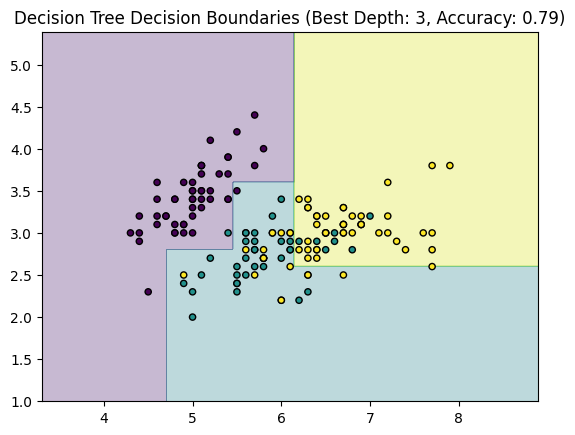
\includegraphics[width=0.7\textwidth]{C/decision-boundary-DT.png}   
\end{figure}
\end{frame}

\begin{frame}[fragile]{Μέρος Γ - Ενότητα 2 - Υλοποίηση - Ερώτημα 1}
Δημιουργούμε ταξινομητή 100 δέντρων με $\gamma = 50\%$.
\lstset{style=python}
\begin{lstlisting}
n_trees = 100
gamma = 0.5  #50% of the training set
n_samples = int(gamma * len(X_train)) 
\end{lstlisting}
Το βάθος του κάθε Δέντρου Απόφασης αποτελεί και πάλι μία υπερπαράμετρο του προβλήματος. 
\lstset{style=python}
\begin{lstlisting}
best_rf_depth = 0
best_rf_accuracy = 0
for depth in range(1, 12):
    rf_clf = RandomForestClassifier(n_estimators=n_trees, max_depth=depth, bootstrap=True, random_state=42, max_samples=gamma)
    rf_clf.fit(X_train, y_train)
    accuracy = rf_clf.score(X_test, y_test)
    if accuracy > best_rf_accuracy:
        best_rf_accuracy = accuracy
        best_rf_depth = depth
\end{lstlisting}
\end{frame}
\begin{frame}{Μέρος Γ - Ενότητα 2 - Υλοποίηση - Ερώτημα 1}
Υλοποιούμε δικό μας ταξινομητή χρησιμοποιώντας την RandomForestClassifier της sklearn και πάλι χρησιμοποιώντας σαν μετρική το accuracy βρίσκουμε το καλύτερο βάθος για το κάθε Δέντρο Απόφασης στο Random Forest μας, έχοντας αναζητήσει σε εύρος τιμών από 1 έως 12.\\
Σε αυτήν την περίπτωση καταλήγουμε πως την καλύτερη ακρίβεια (0.83) την επιτυγχάνουμε για  μέγιστο 2.\\
\vspace{0.3cm}
\textbf{Σχόλιο:} Θα μπορούσαμε να χρησιμοποιήσουμε τη συνάρτηση GridSearchCV της sklearn.model\_selection, την οποία μελετήσαμε και στο εργαστήριο στα πλαίσια του μαθήματος, αφού όμως η συνάρτηση αυτή θα χρησιμοποιηθεί σε μεγάλο βαθμό στο Μέρος Δ, επιλέξαμε να δείξουμε μία διαφορετική λύση στο μέρος αυτό.
\end{frame}
\begin{frame}{Μέρος Γ - Ενότητα 2 - Υλοποίηση - Ερώτημα 2}
Χρησιμοποιώντας όπως μας ζητείται τη συνάρτηση contourf της matplotlib.pyplot απεικονίζουμε τα ζητούμενα όρια απόφασης.
\begin{columns}[c]
    % Left column for the image
    \begin{column}{0.7\textwidth}
        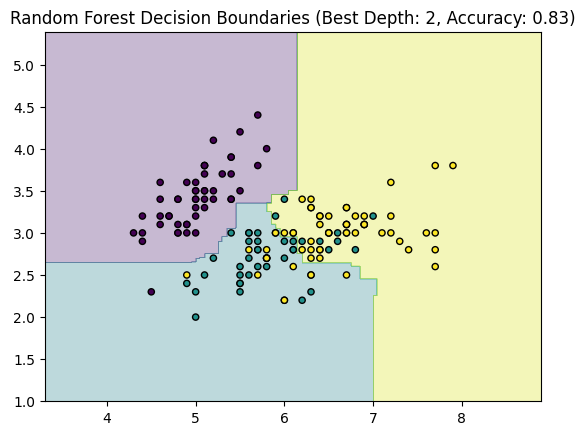
\includegraphics[width=\textwidth]{C/decision-boundary-RF.png}
    \end{column}
    
    % Right column for the text
    \begin{column}{0.33\textwidth}
        Παρατηρούμε πως τα όρια απόφασης έχουν γίνει πιο σύνθετα, και προσαρμόζονται καλύτερα στα δεδομένα, γεγονός που δικαιολογεί και την υψηλότερη ακρίβεια, ίσως όμως ταυτόχρονα να αυξάνεται ο κίνδυνος για overfitting.
    \end{column}
\end{columns}
\end{frame}
\begin{frame}[fragile]{Μέρος Γ - Ενότητα 2 - Υλοποίηση - Ερώτημα 3}
Για να ελέγξουμε την επίδραση του $\gamma$ στην απόδοση του αλγορίθμου, τον εκτελούμε για διάφορες τιμές του. Πιο συγκεκριμένα δοκιμάζουμε 50 τιμές ομοιόμορφα κατανεμημένες στο διάστημα [0.01,1].
\lstset{style=python}
\begin{lstlisting}
gamma_values = np.linspace(0.01, 1, 50)
\end{lstlisting}
Για τα παραπάνω $\gamma$ και για το βέλτιστο βάθος δέντρων παίρνουμε το διάγραμμα που δείχνει την επίδραση του $\gamma$ στη μετρική του accuracy.
\begin{columns}[c]
    % Left column for the image
    \begin{column}{0.63\textwidth}
        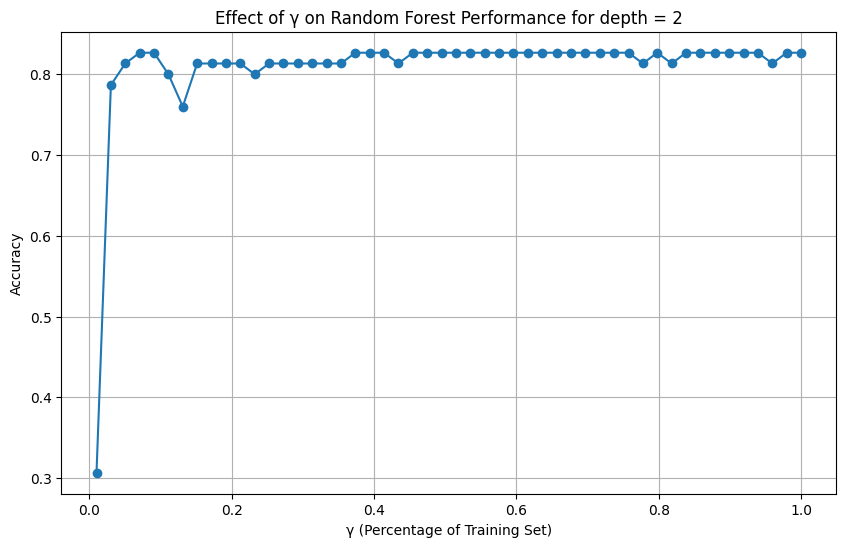
\includegraphics[width=\textwidth]{C/gamma-effect.png}
    \end{column}
    
    % Right column for the text
    \begin{column}{0.33\textwidth}
        Παρατηρούμε πως το $\gamma$ στη συγκεκριμένη περίπτωση δεν επηρεάζει την ακρίβεια πέρα από τιμές που βρίσκονται πολύ κοντά στο 0 ($<0.03$).
    \end{column}
\end{columns}
\end{frame}

\begin{frame}[fragile]{Μέρος Γ - Ενότητα 2 - Υλοποίηση - Ερώτημα 3}
\begin{minipage}[t]{0.49\textwidth} % Top-left
    \centering
    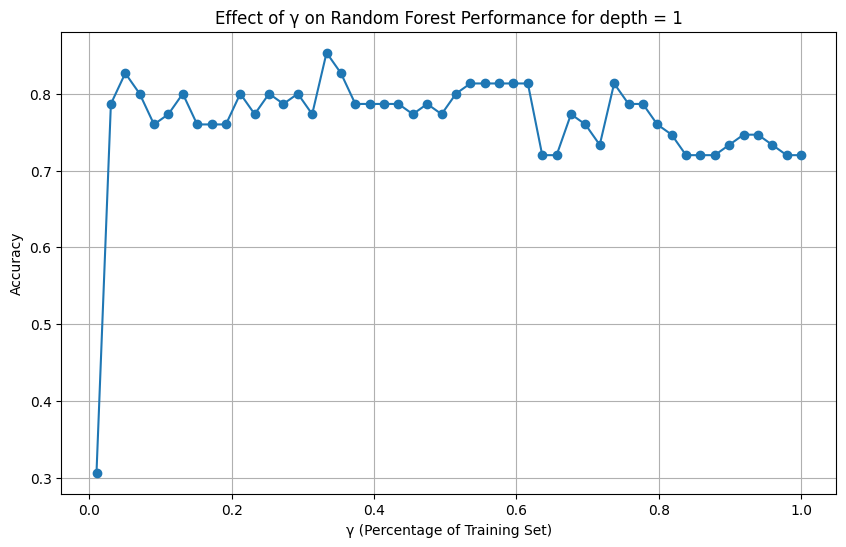
\includegraphics[width=\textwidth]{C/gamma-effect-max-depth_1.png}
\end{minipage}
\hfill
\begin{minipage}[t]{0.49\textwidth} % Top-right
    \centering
    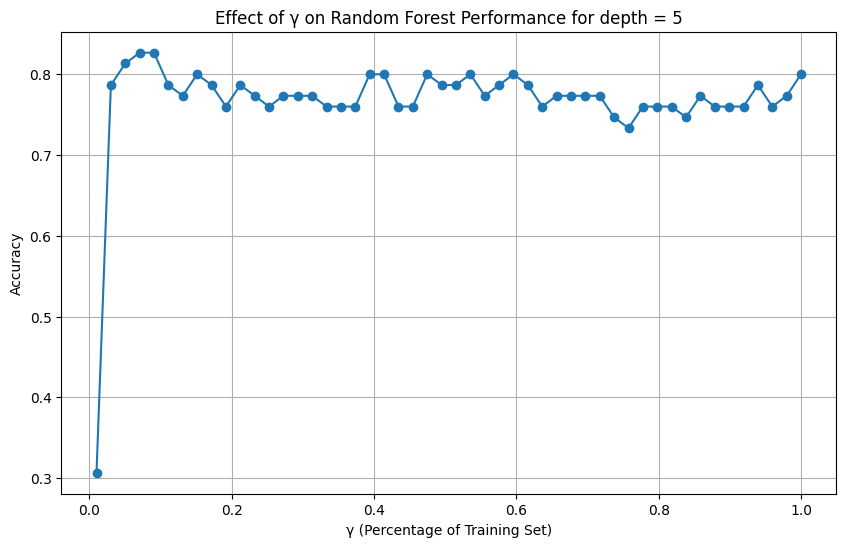
\includegraphics[width=\textwidth]{C/gamma-effect-max-depth_5.png}
\end{minipage}

\begin{minipage}[t]{0.49\textwidth} % Bottom-left
    \centering
    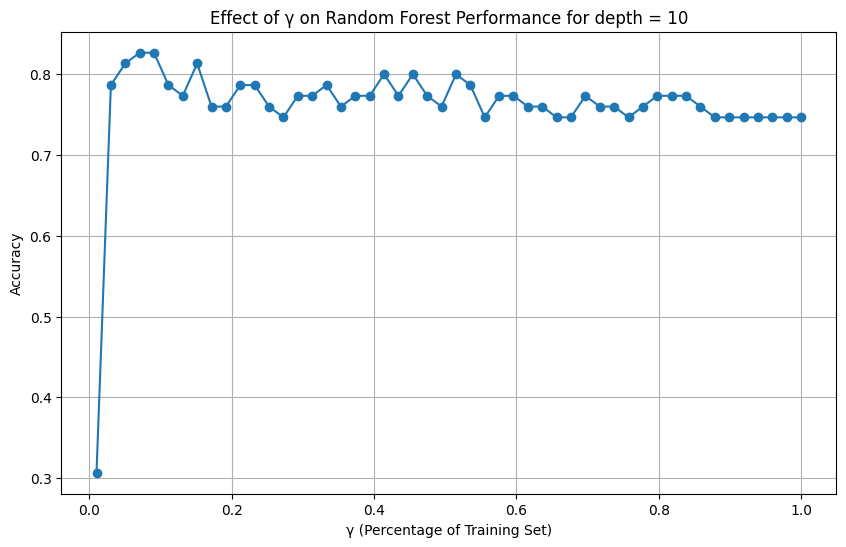
\includegraphics[width=\textwidth]{C/gamma-effect-max-depth_10.png}
\end{minipage}
\hfill
\begin{minipage}[t]{0.49\textwidth} % Bottom-right
    \centering
    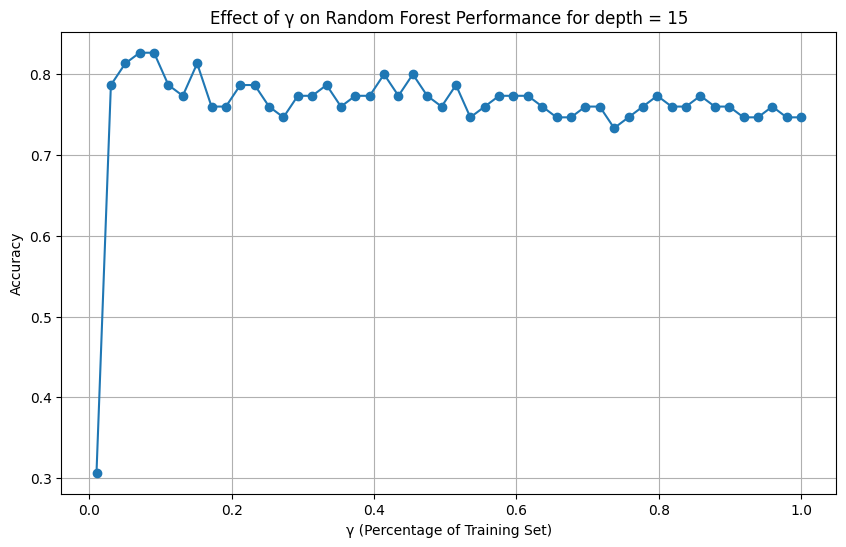
\includegraphics[width=\textwidth]{C/gamma-effect-max-depth_15.png}
\end{minipage}
\end{frame}

\begin{frame}[fragile]{Μέρος Γ - Ενότητα 2 - Ερώτημα 3 - Παρατηρήσεις}
Με βάση τις δύο τελευταίες διαφάνειες μπορούμε να εξάγουμε ορισμένα συμπεράσματα για την επίδραση του $\gamma$:
\begin{itemize}
    \item Παρατηρούμε πως σε κάθε περίπτωση κοντά στο 0 η ακρίβεια πέφτει σημαντικά.
    \item Για μέγιστο βάθος δέντρου 1 υπάρχει μια αρκετά σημαντική επίδραση του $\gamma$ με την υψηλότερη ακρίβεια να επιτυγχάνεται γύρω στο $\gamma = 0.35$, με τιμή ακρίβειας κοντά στο 0.9.
    \item Σε κάθε περίπτωση η ακρίβεια δεν πέφτει κάτω από 0.7 (εξαιρουμένης της περιοχής κοντά στο 0 που αναφέρθηκε προηγουμένως).
    \item Για μεγαλύτερα βάθη συναντάμε την καλύτερη ακρίβεια σε πιο μικρά $\gamma$ γύρω στο 0.1.
\end{itemize}
Συνοψίζοντας η υπερπαράμετρος του $\gamma$ αν και δεν είναι μείζονος σημασίας για τον αλγόριθμο, σίγουρα επηρεάζει σε μικρό βαθμό την ακρίβεια του και απαιτεί μία σύντομη ανάλυση για την εύρεση της βέλτιστης τιμής του, ειδικά σε περιπτώσεις όπου το μέγιστο βάθος των δέντρων δεν είναι το βέλτιστο. 
\end{frame}


\section{Μέρος Δ}
\begin{frame}{Μέρος Δ - Εισαγωγή}
   Στο μέρος Δ καλούμαστε να αναπτύξουμε αλγόριθμο ταξινόμησης με μέθοδο της επιλογής μας. Χρησιμοποιούμε το δοθέν datasetTV.csv ως training set, το οποίο περιέχει 8743 δείγματα με 224 χαρακτηριστικά ανά δείγμα μαζί με τις ετικέτες τους. Επιπλέον, χρησιμοποιούμε το δοθέν datasetTest.csv ως test set για να εφαρμόσουμε το μοντέλο μας και να παράξουμε το ζητούμενο αρχείο - διάνυσμα labels33 με τις προβλέψεις του μοντέλου μας.
\end{frame}

\begin{frame}{Μέρος Δ - Θεωρητική Ανάλυση}
    Η προσέγγιση που επιλέγουμε είναι η εξής:
    \begin{itemize}
        \item Δοκιμάζουμε πολλούς και διαφορετικούς αλγορίθμους που προκύπτουν από διάφορες έτοιμες υλοποιήσεις των βιβλιοθηκών sklearn, xgboost και lightgbm. Δοκιμάζουμε τους: \begin{itemize}
            \item Random Forest (RF)
            \item K-Nearest Neighbors (KNN)
            \item Support Vector Machine (SVM)
            \item Multi-Layer Perceptron (MLP)
            \item Adaptive Boosting (AdaBoost)
            \item Extreme Gradient Boosting (XGBoost)
            \item Light Gradient Boosting Machine (LightGBM)
        \end{itemize}
        \item Χρησιμοποιούμε την GridSearchCV της sklearn για να καταλήξουμε στο βέλτιστο σετ υπερπαραμέτρων για κάθε μοντέλο που επιτυγχάνουν την καλύτερη ακρίβεια στο validation set. Να σημειώσουμε εδώ τα grids που δίνονται παρακάτω είναι ένα υποσύνολο όλων των δοκιμών που έγιναν, για λόγους συντομίας όμως αναφέρουμε τις πιο ουσιώδεις.
    \end{itemize}

\end{frame}

\begin{frame}{Μέρος Δ - Θεωρητική Ανάλυση}
\vspace{-0.2cm}
Κάποιες ακόμα επιλογές μας:
\begin{itemize}
    \item  Πιο συγκεκριμένα, όσο αφορά την GridSearchCV χρησιμοποιούμε cross validation με 3, 5 ή 10 folds και επιλέγουμε το training να γίνει στο 80\% του datasetTV και το validation στο υπόλοιπο 20\%. Οι επιλογές έγιναν με βάση όσα έχουν ειπωθεί στις διαλέξεις και στα εργαστήρια, καθώς και με βάση δική μας έρευνα.
    \item Επιλέγουμε να μην κανονικοποιήσουμε τα δεδομένα μας κατά την προεπεξεργασία γιατί παρατηρούμε πως η κανονικοποίηση είτε με StandardScaler είτε με MinMaxScaler μειώνει την ακρίβεια των προβλέψεων στο validation set. Επιπλέον, ορίζουμε τη συνάρτηση check\_scaling\_or\_normalization που χρησιμοποιεί δείκτες για το range των features και της τυπικής απόκλισης σε ένα δείγμα για να αποφανθούμε αν κάποιο dataset χρήζει κανονικοποίησης.
    \item Χρησιμοποιήσαμε της μετρικές Silhouette Score, Davies-Bouldin Index της sklearn για να έχουμε μία διαισθητική εικόνα των ζητούμενων παραγόμενων labels αν και γνωρίζουμε πως χρησιμοποιούνται ορθότερα σε προβλήματα regression.
        \end{itemize}

\end{frame}


\begin{frame}[fragile]{Μέρος Δ - Random Forest}
Αλγόριθμος γνωστός από το μάθημα. Χρησιμοποιήθηκε η RandomForestClassifier της sklearn.ensemble με την τεχνική Bootstrap που αναλύθηκε και στο μέρος Γ της εργασίας, καθώς παρατηρήσαμε ότι η χρήση της έδινε καλύτερα αποτελέσματα.\\
\textbf{Πλεονεκτήματα:}
\begin{itemize}
    \item Ανθεκτικότητα σε overfitting, λόγω του τρόπου με τον οποίο δημιουργεί και συνδυάζει πολλαπλά ανεξάρτητα decision tree (ensemble, random feature selection).
    \item Αρκετά καλή ακρίβεια σε προβλήματα ταξινόμησης και καταλληλότητα για δεδομένα με πολλά χαρακτηριστικά.
\end{itemize}
\textbf{Μειονεκτήματα:}
\begin{itemize}
    \item Αργός χρόνος εκπαίδευσης και απαίτηση περισσότερων πόρων λόγω της δημιουργίας πολλών δέντρων.
    \item Υψηλό υπολογιστικός κόστος για τη διαδικασία του fine tuning και της εύρεσης των βέλτιστων υπερπαραμέτρων.
\end{itemize}
\end{frame}

\begin{frame}[fragile]{Μέρος Δ - Random Forest}
Δοκιμάστηκαν οι εξής παράμετροι:
\lstset{style=python}
\begin{lstlisting}
# Parameter grid for random forest
param_grid_rf = {
    'n_estimators': [100, 200, 250, 300, 350],
    'max_depth': [None, 1, 2, 5, 7, 10, 20, 25, 30],
    'min_samples_split': [2, 5, 10],
    'min_samples_leaf': [1, 2, 4, 10]
}
\end{lstlisting}
Με βέλτιστες επιλογές να είναι οι:
\begin{itemize}
    \item n\_estimators = 300
    \item max\_depth = None (classifier default value)
    \item min\_samples\_leaf = 1 (classifier default value)
    \item min\_samples\_split = 2 (classifier default value)
\end{itemize}

Η ακρίβεια που επετεύχθη στο validation set ήταν: 0.819325328759291
\end{frame}

\begin{frame}[fragile]{Μέρος Δ - K-Nearest Neighbors}
Αλγόριθμος γνωστός από το μάθημα. Χρησιμοποιήθηκε η KNeighborsClassifier της sklearn.neighbors.\\
\textbf{Πλεονεκτήματα:}
\begin{itemize}
    \item Ευκολία στην εφαρμογή και κατανόηση αφού βασίζεται μόνο στις αποστάσεις μεταξύ των δειγμάτων.
    \item Μπορεί να χρησιμοποιηθεί πολύ αποτελεσματικά σε μικρά datasets και να διαχειριστεί μη γραμμικά δεδομένα.
\end{itemize}
\textbf{Μειονεκτήματα:}
\begin{itemize}
    \item Ευαισθησία σε outliers και σε ενδεχόμενα irrelevant featues.
    \item Δεν κλιμακώνει καλά σε πολύ μεγάλα σύνολα δεδομένων, ειδικά όταν αυξάνεται ο αριθμός των χαρακτηριστικών ή των δειγμάτων.
\end{itemize}
\end{frame}
\begin{frame}[fragile]{Μέρος Δ - K-Nearest Neighbors}
Δοκιμάστηκαν οι εξής παράμετροι:
\lstset{style=python}
\begin{lstlisting}
# Parameter grid for KNN
param_grid_knn = {
    'n_neighbors': [5, 7, 9, 11, 13, 15],
    'weights': ['uniform', 'distance'], 
    'metric': ['euclidean', 'manhattan', 'minkowski'],
}
\end{lstlisting}
Ο αριθμός των γειτόνων επιλέγεται ως περιττός αριθμός για να μην υπάρχουν ισοπαλίες σε διαδικασίες classification.\\
Βέλτιστες επιλογές είναι οι:
\begin{itemize}
    \item n\_neighbors = 7
    \item weights = 'distance' 
    \item metric = 'euclidean' (classifier default value)
\end{itemize}

Η ακρίβεια που επετεύχθη στο validation set ήταν: 0.8467695826186392
\end{frame}

\begin{frame}[fragile]{Μέρος Δ - Support Vector Machine}
Αλγόριθμος γνωστός από το μάθημα. Χρησιμοποιήθηκε η  SVC (Support Vector Classifier) της sklearn.svm. \\
\textbf{Πλεονεκτήματα:}
\begin{itemize}
    \item Υψηλή αποτελεσματικότητα σε δεδομένα υψηλή διάστασης, λόγω της χρήσης του kernel και της εκ κατασκευής μεγιστοποίησης του περιθωρίου μεταξύ των κλάσεων.
    \item Πολύ καλή ικανότητα γενίκευσης και δυνατότητα αποφυγής overfitting, ειδικά όταν το μέγεθος του dataset είναι περιορισμένο.
\end{itemize}
\textbf{Μειονεκτήματα:}
\begin{itemize}
    \item Αυξημένη υπολογιστική πολυπλοκότητα ειδικά για μεγάλα datasets, και κατά τη διάρκεια αναζήτησης των βέλτιστων υπερπαραμέτρων.
    \item Υπάρχει μεγάλη ευαισθησία στην επιλογή των υπερπαραμέτρων, αν δεν γίνει σωστή επιλογή του kernel, του C και του gamma ο αλγόριθμος μπορεί να μην αποδώσει.
\end{itemize}
\end{frame}
\begin{frame}[fragile]{Μέρος Δ - Support Vector Machine}
Δοκιμάστηκαν οι εξής παράμετροι:
\lstset{style=python}
\begin{lstlisting}
# Parameter grid for SVM
param_grid_svm = {
    'C': [0.1, 1, 8, 9, 10, 11, 12, 15, 100],
    'gamma': [1, 0.1, 0.03, 0.025, 0.022, 0.02, 0.018, 0.015, 0.01, 0.001],
    'kernel': ['linear', 'rbf']
}
\end{lstlisting}

Βέλτιστες επιλογές είναι οι:
\begin{itemize}
    \item C = 9
    \item gamma = 0.025
    \item kernel = 'rbf' (classifier default value)
\end{itemize}
Η ακρίβεια που επετεύχθη στο validation set ήταν: 0.873642081189251
\end{frame}

\begin{frame}[fragile]{Μέρος Δ - Multi-Layer Perceptron}
Αλγόριθμος ενός feedforward νευρωνικού δικτύου γνωστός από το μάθημα. Χρησιμοποιήθηκε η MLPClassifier της sklearn.neural\_network. \\
\textbf{Πλεονεκτήματα:}
\begin{itemize}
    \item Universal Approximator, όπως είδαμε και στο μάθημα μπορεί να προσεγγίσει αρκετά καλά οποιαδήποτε συνάρτηση με αρκετούς νευρώνες.
    \item Προσφέρει μία σχετική ευελιξία αφού υπάρχουν πολλές δυνατότητες επιλογής της αρχιτεκτονικής του, οι οποίες κλιμακώνουν καλά σε μεγαλύτερα datasets αν υπάρχουν πόροι. 
\end{itemize}
\textbf{Μειονεκτήματα:}
\begin{itemize}
    \item Απαιτείται πολύ μεγάλη υπολογιστική ισχύς ειδικά για μεγάλα datasets.
    \item Κίνδυνος overfitting αν δεν υπάρχει ικανός αριθμός από δεδομένα.
\end{itemize}
\end{frame}
\begin{frame}[fragile]{Μέρος Δ -  Multi-Layer Perceptron}
\vspace{-0.3cm}
Δοκιμάστηκαν οι εξής παράμετροι:
\lstset{style=python}
\begin{lstlisting}
# Parameter grid for MLP
param_grid_mlp = 
{   'hidden_layer_sizes': [(10), (100), (50,50), (100,50), (100,100), (50,50,50), (400, 40), (400,38), (400,42)],
    'activation': ['tanh', 'relu'],         
    'solver': ['sgd', 'adam'],                   
    'alpha': [0.0001, 0.001, 0.01],                    
    'learning_rate': ['constant', 'adaptive'],        
    'learning_rate_init': [0.001, 0.01],       }
\end{lstlisting}

Βέλτιστες επιλογές είναι οι:
\begin{itemize}
    \item hidden\_layer\_sizes = (400,40)
    \item activation = 'relu' ( classifier default value)
   \item solver = 'adam' (classifier default value)
    \item alpha = 0.001 (classifier default value)
    \item learning\_rate = 'constant' (classifier default value)
    \item learning\_rate\_init = 0.001 (classifier default value)
\end{itemize}
Η ακρίβεια που επετεύχθη στο validation set ήταν: 0.855917667238422
\end{frame}

\begin{frame}[fragile]{Μέρος Δ - Adaptive Boosting}
Αλγόριθμος γνωστός από το μάθημα. Χρησιμοποιήθηκε η AdaBoostClassifier της sklearn.ensemble.\\
\textbf{Πλεονεκτήματα:}
\begin{itemize}
    \item Δίνει μεγαλύτερη έμφαση στα δείγματα που ταξινομούνται λανθασμένα (Boosting), βελτιώνοντας τη συνολική απόδοση.
    \item Μπορεί να συνδυαστεί με διάφορους αλγορίθμους (π.χ., decision stumps, decision trees) και είναι σχετικά εύκολο να εφαρμοστεί, καθώς οι βασικοί αλγόριθμοι λειτουργούν αυτόνομα και εστιάζουν μόνο στις αδύναμες περιοχές.
\end{itemize}
\textbf{Μειονεκτήματα:}
\begin{itemize}
    \item Ο διαδοχικός τρόπος με τον οποίο εκπαιδεύονται τα weak learners (με ενημέρωση των βαρών σε κάθε βήμα) μπορεί να είναι πιο αργός σε σχέση με άλλους αλγορίθμους, ειδικά σε μεγάλα datasets.
    \item Ενδέχεται να επηρεαστεί σε μεγάλο βαθμό από outliers, καθώς τους δίνει μεγαλύτερη σημασία στις επόμενες επαναλήψεις.
\end{itemize}
\end{frame}
\begin{frame}[fragile]{Μέρος Δ -  Adaptive Boosting}
Δοκιμάστηκαν οι εξής παράμετροι:
\lstset{style=python}
\begin{lstlisting}
# Parameter grid for AdaBoost
param_grid_ab = {
    'n_estimators': [50, 100, 200, 300],
    'learning_rate': [0.01, 0.1, 1, 10]
}

\end{lstlisting}

Βέλτιστες επιλογές είναι οι:
\begin{itemize}
    \item n\_estimators = 300
    \item learning\_rate = 0.1

\end{itemize}
Η ακρίβεια που επετεύχθη στο validation set ήταν: 0.6958261863922242
\end{frame}



\begin{frame}[fragile]{Μέρος Δ - Gradient Boosting}
Διαισθητικά ένας Gradient Boosting αλγόριθμος, συνδυάζει δύο τεχνικές γνωστές από το μάθημα, αυτή του Boosting, δηλαδή τον συνδυασμό πολλών weak learners σε έναν πιο "ισχυρό" learner, στον οποίο σε κάθε επάναληψη διορθώνονται τα "λάθη" των προγόνων, με αυτή του Gradient Desecent. Ο αλγόριθμος συνοπτικά:

\begin{minipage}[t]{\textwidth}
\centering
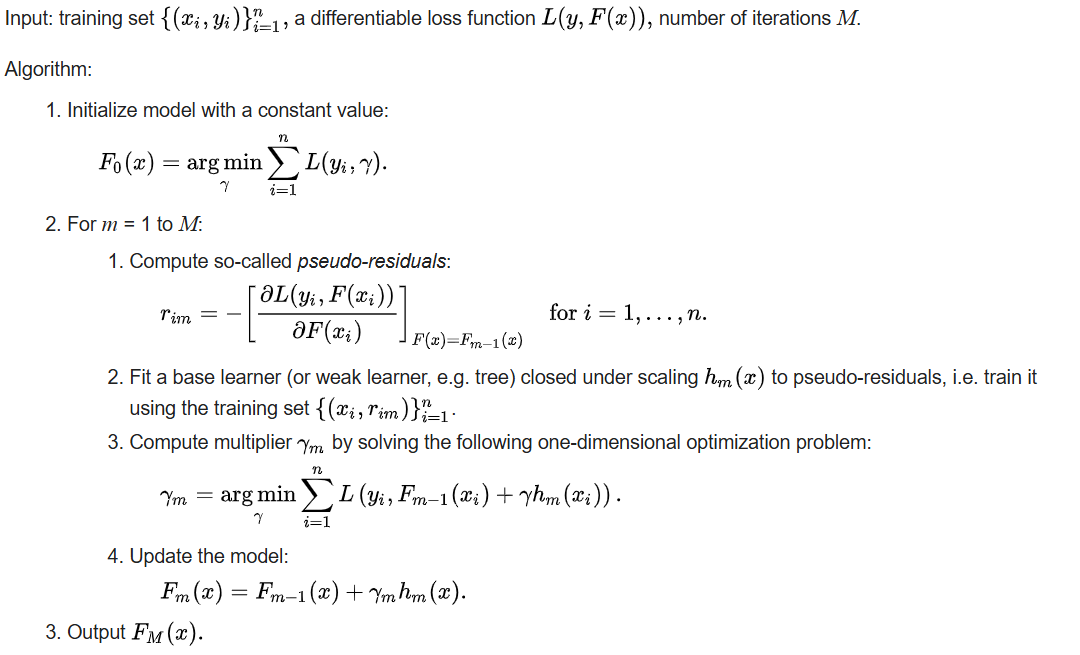
\includegraphics[width=0.75\textwidth]{gradient boosting.png}  
\end{minipage}
\end{frame}

\begin{frame}[fragile]{Μέρος Δ - Extreme Gradient Boosting}
Ο XGBoost αποτελεί μια βελτιωμένη υλοποίηση του Gradient Boosting, με τεχνικές κανονικοποίησης, παραλληλισμού, και βελτιστοποιήσεις για ταχύτητα και ακρίβεια, καθιστώντας τον ιδανικό για μεγάλα και σύνθετα datasets. Χρησιμοποιήθηκε η XGBClassifier της xgboost.\\
\textbf{Πλεονεκτήματα:}
\begin{itemize}
    \item Υψηλή ακρίβεια γιατί συνδυάζει τεχνικές κανονικοποίησης, early stopping, και παραμετροποίηση, καθιστώντας τον ιδιαίτερα αποδοτικό για datasets με σύνθετα μοτίβα.
    \item Πλήρης υποστήριξη παραλληλισμού κατά την εκπαίδευση, επιταχύνοντας τη διαδικασία σε μεγάλα datasets, ενώ μπορεί να διαχείριστει με υψηλή ακρίβεια task παλινδρόμησης, ταξινόμησης και βαθμολόγησης.
\end{itemize}
\textbf{Μειονεκτήματα:}
\begin{itemize}
    \item Απαίτηση για μεγάλη υπολογιστική ισχύς και μνήμη, ιδιαίτερα σε μεγάλα datasets.
    \item Πολύ μεγάλος αριθμός υπερπαραμέτρων και έτσι η διαδικασία εύρεσης των βέλτιστων γίνεται πολύ σύνθετη και χρονοβόρα.
\end{itemize}
\end{frame}
\begin{frame}[fragile]{Μέρος Δ - Extreme Gradient Boosting}
Δοκιμάστηκαν οι εξής παράμετροι:
\lstset{style=python}
\begin{lstlisting}
# Parameter grid for XGB
param_grid_xgb = {
    'n_estimators': [50, 100, 200, 300],
    'learning_rate': [0.01, 0.1, 0.2, 0.3],
    'max_depth': [3, 5, 7, 10],
    'subsample': [0.7, 0.8, 0.9, 1.0],
    'colsample_bytree': [0.7, 0.8, 0.9, 1.0]
}

\end{lstlisting}

Βέλτιστες επιλογές είναι οι:
\begin{itemize}
    \item n\_estimators = 300
    \item learning\_rate = 0.1
    \item max\_depth = 7
    \item subsample = 0.7
    \item colsample\_bytree = 0.7
\end{itemize}
Η ακρίβεια που επετεύχθη στο validation set ήταν: 0.8502001143510578
\end{frame}



% \begin{frame}[fragile]{Μέρος Δ - Light Gradient Boosting Machine}
% ΕΞΗΓΗΣΗ ΜΑΘΗΜΑΤΙΚΑ ΚΑΙ ΣΚΕΠΤΙΚΟ ΑΛΓΟΡΙΘΜΟΥ
% \end{frame}

\begin{frame}[fragile]{Μέρος Δ - Light Gradient Boosting Machine}
\vspace{-0.1cm}
Ο LightGBM είναι ένας ελαφρύς και εξαιρετικά αποδοτικός αλγόριθμος Gradient Boosting που χρησιμοποιεί histogram-based προσέγγιση (διακριτοποίηση των συνεχών χαρακτηριστικών σε ομάδες (bins) πριν από την αναζήτηση των βέλτιστων splits) και τεχνικές όπως το leaf-wise growth, βελτιώνοντας την απόδοση σε μεγάλα σύνολα δεδομένων με πολλές διαστάσεις. Χρησιμοποιήθηκε η LGBMClassifier της lightgbm.
\textbf{Πλεονεκτήματα:}
\begin{itemize}
    \item Η histogram-based προσέγγιση για την κατασκευή δέντρων απόφασης μειώνει σημαντικά τον χρόνο εκπαίδευσης σε σύγκριση με άλλους αλγορίθμους Gradient Boosting.
    \item  Η ανάπτυξη δέντρων με βάση τα φύλλα (leaf-wise) ενδέχεται να οδηγήσει σε μεγαλύτερη ακρίβεια σε σύνθετα datasets, σε σχέση με άλλους αλγορίθμους.
\end{itemize}
\textbf{Μειονεκτήματα:}
\begin{itemize}
    \item Η ανάπτυξη δέντρων με βάση τα φύλλα ίσως προκαλεί overfitting.
    \item Πολύ μεγάλος αριθμός υπερπαραμέτρων και έτσι η διαδικασία εύρεσης των βέλτιστων γίνεται πολύ σύνθετη και χρονοβόρα.
\end{itemize}
\end{frame}
\begin{frame}[fragile]{Μέρος Δ - Light Gradient Boosting Machine}
Δοκιμάστηκαν οι εξής παράμετροι:
\lstset{style=python}
\begin{lstlisting}
# Parameter grid for lightGBM
param_grid_lgbm = {
    'num_leaves': [31, 50, 70, 100, 150, 300],
    'max_depth': [-1, 10, 20],         
    'learning_rate': [0.01, 0.05, 0.1, 0.15, 0.2], 
    'n_estimators': [100, 150, 200, 250, 300, 500],   
    'min_child_samples': [10, 20, 30], 
    'subsample': [0.8, 1.0]    }
\end{lstlisting}

Βέλτιστες επιλογές είναι οι:
\begin{itemize}
    \item num\_leaves =31 (classifier default value)
    \item max\_depth =-1 (classifier default value)
    \item learning\_rate = 0.1 (classifier default value)
    \item n\_estimators = 200
    \item min\_child\_samples = 20 (classifier default value)
    \item subsample = 0.8
\end{itemize}
Η ακρίβεια που επετεύχθη στο validation set ήταν: 0.8444825614636935
\end{frame}

\begin{frame}{Μέρος Δ - Σύνοψη των αποτελεσμάτων}
   Παρουσιάζονται σε μορφή πίνακα η ακρίβεια στο validation set για όλα τα μοντέλα που δοκιμάστηκαν:
    \begin{table}[h!]
\centering
\begin{tabular}{|l|c|}
\hline
\textbf{Αλγόριθμος} & \textbf{Accuracy} \\ \hline
Random Forest (RF) & 0.819325328759291\\ \hline
K-Nearest Neighbors (KNN) & 0.8467695826186392\\ \hline
\textbf{Support Vector Machine (SVM)} & \textbf{0.873642081189251}\\ \hline
Multi-Layer Perceptron (MLP) & 0.855917667238422\\ \hline
Adaptive Boosting (AdaBoost) & 0.6958261863922242\\ \hline
Extreme Gradient Boosting (XGBoost) & 0.8502001143510578 \\ \hline
Light Gradient Boosting Machine (LightGBM) & 0.8444825614636935\\ \hline
\end{tabular}

\end{table}
\end{frame}

\begin{frame}{Μέρος Δ - Το τελικό Μοντέλο}
    Η λύση που προτείνουμε με βάση τις παραπάνω μετρικές είναι η εξής:
    \begin{itemize}
        \item \textbf{Αλγόριθμος:} Support Vector Machine (SVM)
        \item \textbf{Υπερπαράμετροι:} 
            \begin{itemize}
                \item C = 9
                \item gamma = 0.025
                \item kernel = 'rbf'
            \end{itemize}
        \item \textbf{Accuracy στο validation set:} 0.873642081189251
    \end{itemize}
    Τρέχοντας τα 3 πρώτα κελιά του αρχείου Team33-D.ipynb παράγεται το αρχείο labels33.npy με τα ζητούμενα labels.
\end{frame}
\section{Πηγές}
\begin{frame}{Πηγές}
\begin{itemize}
    \item   \url{https://en.wikipedia.org/wiki/Gradient_boosting}
    \item  \url{https://web.archive.org/web/20191101082737/http://statweb.stanford.edu/~jhf/ftp/trebst.pdf}
    \item \url{https://lightgbm.readthedocs.io/}
    \item \url{https://xgboost.readthedocs.io/}
    \item  \url{https://scikit-learn.org/}
\end{itemize}

  
    
\end{frame}




\end{document}
